
\documentclass[review]{elsarticle}

\usepackage{lineno,hyperref,color}
\modulolinenumbers[5]

\journal{Nuclear Instruments and Methods B}

%%%%%%%%%%%%%%%%%%%%%%%
%% Elsevier bibliography styles
%%%%%%%%%%%%%%%%%%%%%%%
%% To change the style, put a % in front of the second line of the current style and
%% remove the % from the second line of the style you would like to use.
%%%%%%%%%%%%%%%%%%%%%%%

%% Numbered
%\bibliographystyle{model1-num-names}

%% Numbered without titles
%\bibliographystyle{model1a-num-names}

%% Harvard
%\bibliographystyle{model2-names.bst}\biboptions{authoryear}

%% Vancouver numbered
%\usepackage{numcompress}\bibliographystyle{model3-num-names}

%% Vancouver name/year
%\usepackage{numcompress}\bibliographystyle{model4-names}\biboptions{authoryear}

%% APA style
%\bibliographystyle{model5-names}\biboptions{authoryear}

%% AMA style
%\usepackage{numcompress}\bibliographystyle{model6-num-names}

%% `Elsevier LaTeX' style
\bibliographystyle{elsarticle-num}
%%%%%%%%%%%%%%%%%%%%%%%

\begin{document}

\begin{frontmatter}

\title{Radiation damage of scintillator rods with different concentrations of dopants
}


%% or include affiliations in footnotes:
\author[umd]{Geng-Yuan Jeng\corref{mycorrespondingauthor}}
\cortext[mycorrespondingauthor]{Corresponding author}
\ead{Geng-Yuan.Jeng@cern.ch}
\author[umd]{A. Belloni}
\author[umd]{Shiyuan Duan}
\author[umd]{S. Eno}
\author[umd]{T. Edberg}
\author[umd]{C, Hinrich}
\author[umd]{C. Papageorgakis}
\author[umd]{Ruhi Perez}
\author[umd]{Cameron Sylber}
\author[umd]{Zishuo Yang}
\author[umd]{Yao Yao}
\author[umd]{Yingyue Zhu}

\address[umd]{Dept. Physics, U. Maryland, College Park MD 30742 USA}



\begin{abstract}
The performance of plastic scintillator degrades when exposed to radiation. 
In this paper, the reduction in light output  as a function of dose rate
is studied for scintillators
with varying concentrations of the primary dopant, secondary dopant

The scintillators used polystyrene or polyvinyltoluene as the substrate, and
produced blue or green light. \textcolor{red}{some findings here}
\end{abstract}

\begin{keyword}
organic scintillator\sep radiation hardness \sep calorimetry
\end{keyword}

\end{frontmatter}

\linenumbers

\section{Introduction}
Plastic scintillator has long been an inexpensive way to detect charged particles produced in particle physics experiments.
They consist of a plastic substrate, 
often polystyrene (PS) or polyvinyltoluene (PVT),
into which wavelength 
shifting primary and secondary fluors have been dissolved.
When a charged particle traverses the scintillator, the molecules of the substrate are excited.  
This excitation can be transferred to the primary fluor radiatively in the deep UV at low concentrations or via the F{\"o}rster 
mechanism~\cite{forster} at concentrations above $\approx$ 1\%~\cite{birks}.  
The primary fluor transfers the excitation radiatively to the secondary fluor.  
The visible light by de-excitation of the secondary flour
must traverse the scintillator to reach a photodetector, and can be absorbed by ``color centers'' along its path.


Prolonged exposure of plastic scintillator to
ionizing radiation, however, can result in damage:
light self-absorption by the color centers (yellowing) increases when the radicals created during irradiation re-terminate in ways that absorb visible light.
The transfer efficiency of the initial excitation of the polymer to the
dopants combined with the probability of radiative decays for the dopants (``initial light output'') can lessen
when bonds form that absorb in the ultraviolet.

The effect of radiation on plastic scintillator is known to depend
both on dose and dose rate ~\cite{sauli,34504,Wick1991472,289295,173180,173178,Giokaris1993315,gillen,1748-0221-11-10-T10004}.  
Two well-studied~\cite{clough1,bolland1,bolland2,bateman,cunliffe,Wick1991472,Biagtan1996125}
sources of dose rate effects in plastics
involve oxygen.   The penetration depth of oxygen
during irradiation depends on the dose rate.
The rate of peroxide
formation in the areas containing oxygen can as well~\cite{clough1}.
At low enough dose rate, oxygen permeates the plastic 
and the radicals created during irradiation tend to quickly
form peroxides that absorb in the ultraviolet~\cite{clough1}, affecting the initial light output.  
The rate of peroxide formation may depend on the dose rate if the bond formed is bimolecular.
At high enough dose rate, however, the penetration depth for oxygen may
be thinner than the thickness of the plastic, and many short-lived ``temporary'' color centers can form in the oxygen-free regions.  
These color centers anneal after irradiation either by reforming bonds or by forming peroxides when oxygen re-permeates the plastic.
Because of this, dose rate effects might be ameliorated either by increasing the concentration of the dopant to shorten the path length for the ultraviolet light to the primary dopant.


In this paper, we present measurements of the light output 
of blue and green scintillator rods 
before and after irradiation for various concentrations of dopants, and
as a function of the material used for the substrate.
The damage is studied for 
for dose rates from \textcolor{red}{xxx to xxx}.


\section{Sample and irradiation details}
The rods were supplied by Eljen Corporation, and
are similar to EJ-200, a blue scintillator, and EJ-260, a green one, using either
PS or PVT as the substrate.
They are rectangular, with dimensions of 1x1x5~$\rm{cm^3}$, 
and the edges were diamond milled.
The concentration of the primary dopant and the secondary dopant
was 0.5, 1.0, and 2.0 times the nominal concentration.
Fig.~\ref{fig:fg} [left] shows a photograph of some of the rods.

High dose rate irradiations \textcolor{red}{( xxx--xxx~krad/hr)}
were performed at the National Institute of Standards and Technology, Gaithersburg, MD, using their Cobalt-60 (Co-60) source.  Intermediate dose rate irradiations (\textcolor{red}{xxx--xxx~krad/hr}) were performed at Goddard Space Flight Center's Co-60 source.  Very low dose rate were measured using the GIF++ facility\cite{gif} at CERN.  The source is \textcolor{red}{Cs-137?} and the dose rate \textcolor{red}{xxx~krad/hr}.

\section{Measurement technique}
The light output from the rods is measured before and after
irradiation using an alpha source, as shown in Fig.~\ref{fig:hd} [right].
Before measurement, the rods were allowed to anneal
at least 2 months,  until all the temporary damage was gone.
The rod is placed on a Hamamatsu \textcolor{red}{RXXX} PMT, and the
source is placed on the rod.  An alignment jig ensures reproducibility
of the alignment of the three pieces.  The measurements were made using
a \textcolor{red}{textronics scope XXXXX}, with a charge integration
window of \textcolor{red}{xx$\mu s$}.
A typical output spectrum is shown in Fig.~\ref{fig:hd} [right].
The distribution is fit to a Gaussian near the peak, and its mean is used as a measure of the light yield.  The uncertainty in the light output is taken as the variation in this mean for measurements taken at different times, and after removing and replacing the rod from the jig, and is
\textcolor{red}{$\pm 2$\%}.

\begin{figure}[hbtp]
\centering
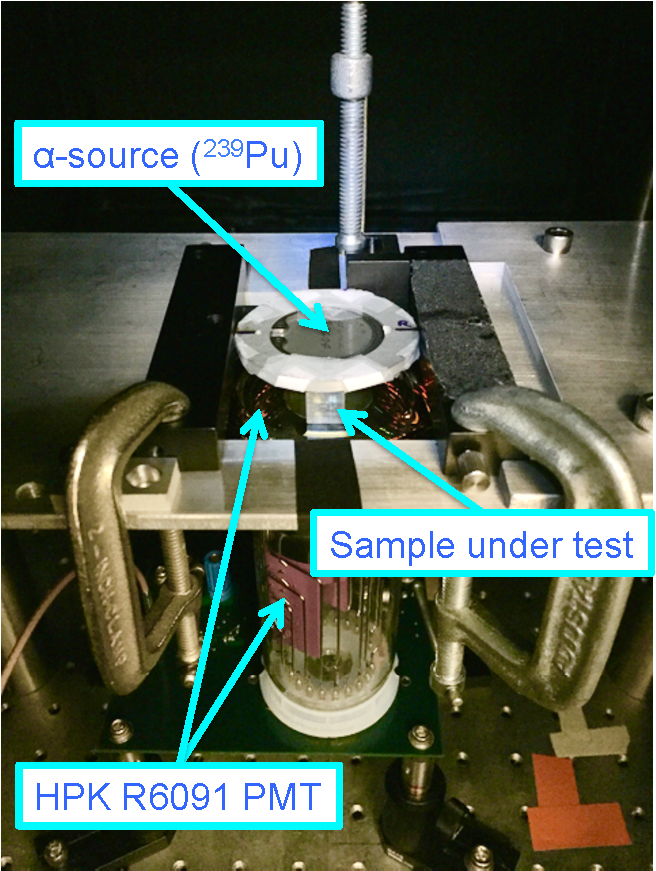
\includegraphics[width=0.25\textwidth]{Setup_AlphaSource.pdf}
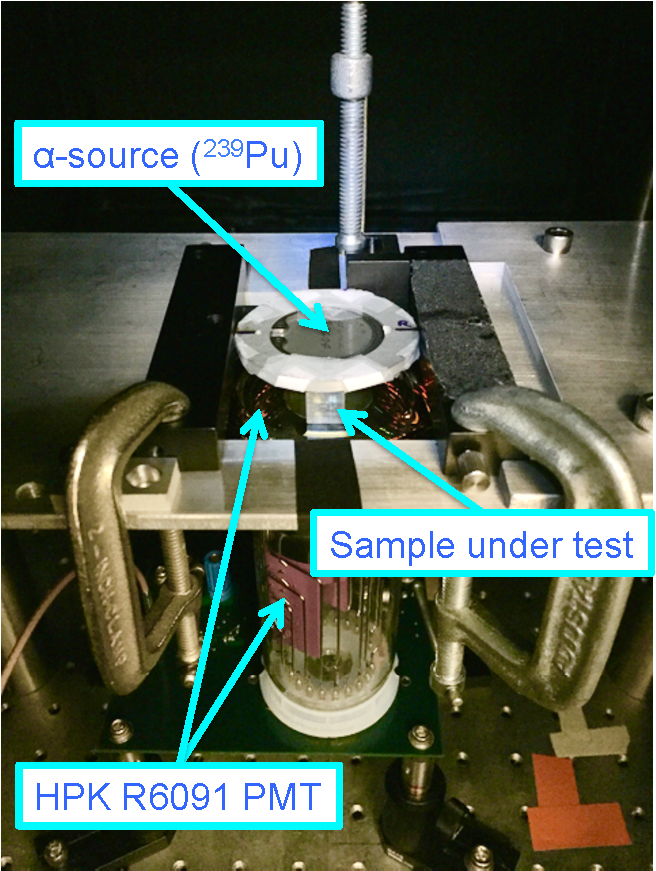
\includegraphics[width=0.25\textwidth]{Setup_AlphaSource.pdf}
\caption{
[left] photograph of some of the rods
[right] Apparatus for measurements with alpha source.
}
  \label{fig:hd}
\end{figure}

The amount of radiation damage is quantified 
using $D$ defined in Equation~\ref{eqn:exp}.
\begin{equation}
\frac{L(d)}{L_0}=\exp{-d/D}
\label{eqn:exp}
\end{equation}
where $L(d)$ is the light output after a dose $d$, $L_0$ is the initial light
output, and $D$ is the exponential dose constant from the fit.


\section{Results}


\begin{figure}[hbtp]
\centering
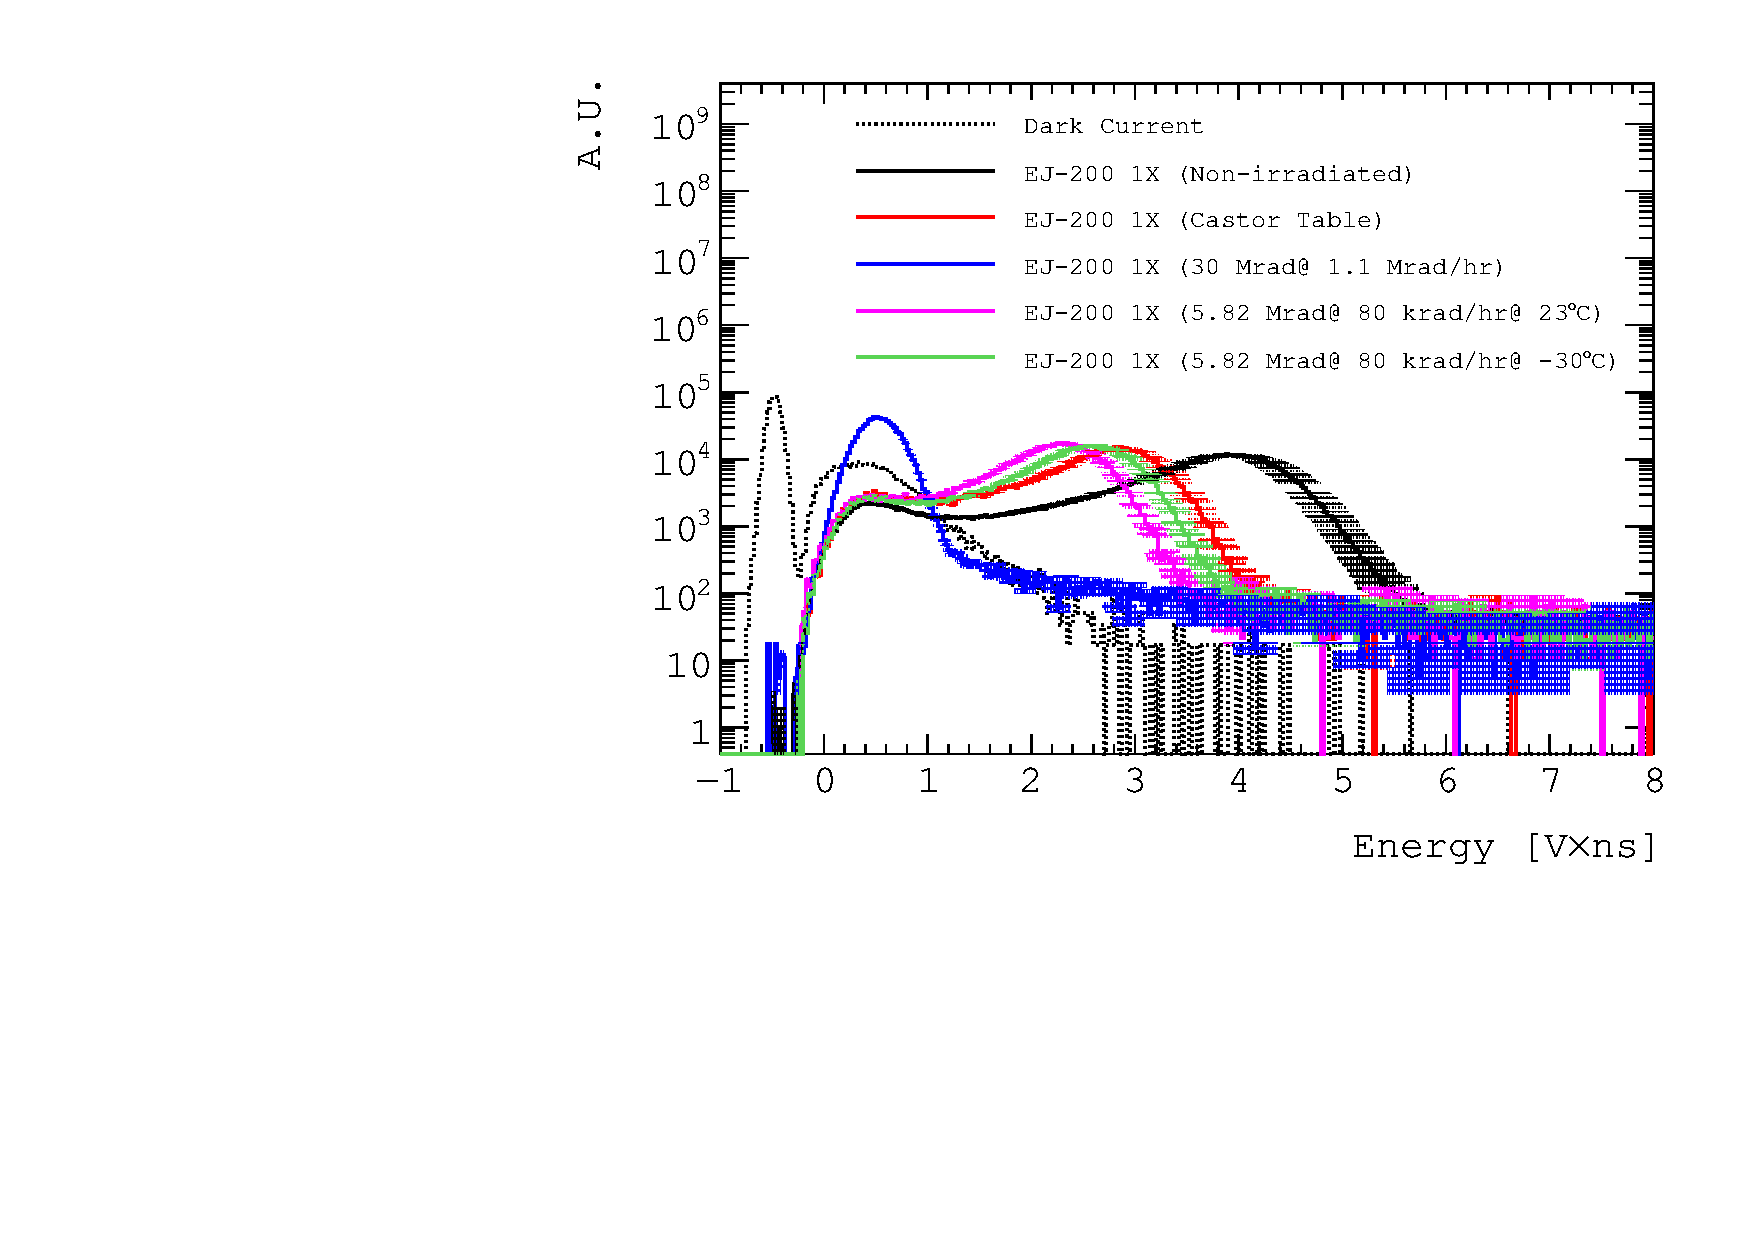
\includegraphics[width=0.45\textwidth]{AlphaSourceMeasurement-EJ200OLD_nominal.pdf}
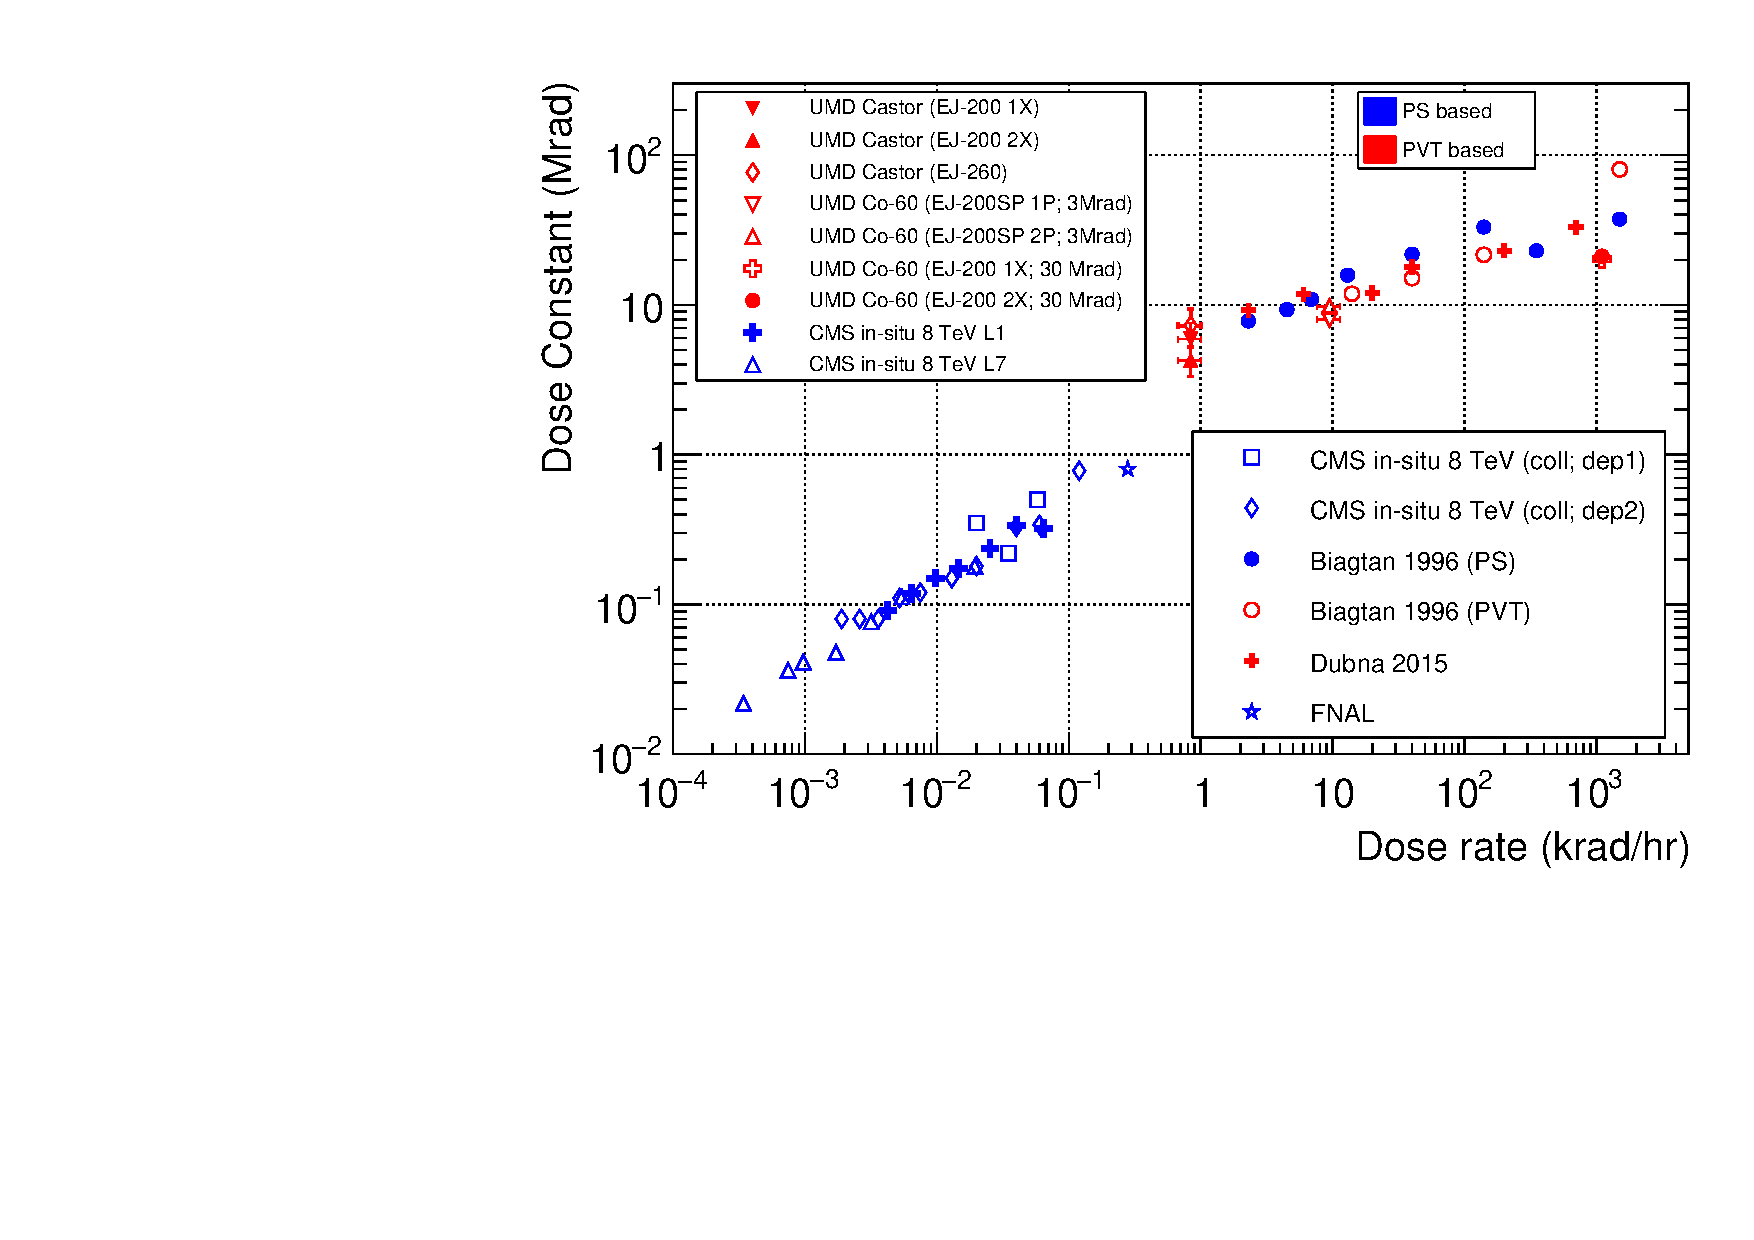
\includegraphics[width=0.45\textwidth]{DoseConstVsDoseRate}
    \caption{
[left] A typical energy spectrum 
[right] resulting dose constants and comparison with the HE data. \textcolor{red}{need version without HE data}
    }
    \label{fig:GY_more2}
\end{figure}




\section{Conclusions}

\section{Acknowledgments}
The authors would like to thank Chuck Hurlbut of Eljen Corporation for supplying many of the rods.
The authors would like to thank the staff
Goddard Space Flight Center and at the National Institute of Standards and Technology irradiation
Facilities group for assistance
with the irradiations. 
This work was supported in part by U.S. Department of Energy Grant DESC0010072.

\section*{References}

\bibliography{atiledopings}

\end{document}
